\section{Basic Concepts}
\subsection{Quantum bits (qubits)}

Classical bits: $0, 1$ \newline
Quantum bit \textit{qubit}: Superposition of $0$ and $1$:

A quantum state $\ket{\psi}$ is described as 
\begin{equation}
    \ket{\psi} := \alpha \ket{0} + \beta \ket{1}, \quad \alpha, \beta \in \mathbb{C} 
\end{equation}
where 
\begin{equation}
    \abs{\alpha}^2 + \abs{\beta}^2 = 1 \quad \text(normalization).
\end{equation}
%
Mathematical description: $\ket{\psi} \in \mathbb{C}^2$ with
\begin{equation*}
    \ket{0} = \begin{pmatrix}1 \\ 0 \end{pmatrix}, 
    \quad \ket{1} = \begin{pmatrix}0 \\ 1\end{pmatrix}
    \quad \leadsto \ket{\psi} = \begin{pmatrix}
        \alpha \\ \beta
    \end{pmatrix}
\end{equation*}


Different from classical bits, cannot (in general) directly observe / measure a qubit 
(the amplitudes $\alpha$ and $\beta$).
%
Instead: "\textit{standard}" measurement will result in 
\begin{itemize}
    \item $0$ with probability $\abs{\alpha}^2$
    \item $1$ with probability $\abs{\beta}^2$
\end{itemize}
%

The measurement also \underline{changes} the qubit (\textit{wavefunction collapse}).
%
If measuring $0$, the qubit will be $\ket{\psi} = \ket{0}$ directly after the measurement,
and likewise if measuring $1$, the qubit will be $\ket{\psi} = \ket{1}$. \newline

In practise: Can estimate the probabilities $\abs{\alpha}^2$ and $\abs{\beta}^2$ in 
experiments by repeating the same experiment many times (i.e via outcome statistics).
These repetitions are called \textit{trials} or \textit{shots}.

\begin{figure}[h]
    \centering
    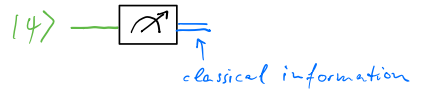
\includegraphics[scale=0.5]{chapters/res/circuit-notation.png}
    \caption{Circuit notation}
\end{figure}
\newpage

A useful graphical deputation of a qubit is the \underline{Bloch sphere} representation:
If $\alpha$ and $\beta$ happen to be real-valued, then can find angle 
$\vartheta \in \mathbb{R}$ such that
\begin{equation}
    \alpha = \cos{\frac{\vartheta}{2}}, \quad \beta = \sin{\frac{\vartheta}{2}}
\end{equation}
\begin{equation*}
    (\leadsto \abs{\alpha}^2 + \abs{\beta}^2 
    = \cos{\frac{\vartheta}{2}} + \sin{\frac{\vartheta}{2}}) = 1 \quad \color{green}\checkmark
\end{equation*}

\begin{figure}[h]
    \centering
    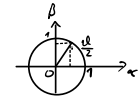
\includegraphics[scale=0.5]{chapters/res/bloch_sphere_sin_cos.png}
\end{figure}

In general: represent 
\begin{align*}
    \alpha &= e^{i \gamma} \cos{\frac{\vartheta}{2}} \\
    \beta &= e^{i (\varphi + \gamma)} \sin{\frac{\vartheta}{2}} \\
\end{align*}
using so-called phase angles $\gamma$ for $\alpha$ and $\varphi + \gamma$ for $\beta$.

\begin{figure}[h]
    \centering
    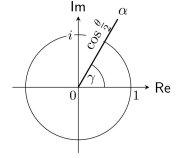
\includegraphics[scale=0.6]{chapters/res/sin-cos-complex.png}
\end{figure}

Then:
\begin{align}
    \ket{\psi} &= 
        e^{i \psi} \cos{\frac{\vartheta}{2}} \cdot \ket{0} 
        + \underbrace{e^{i (\varphi + \gamma)}}_{= \text{ } e^{i\varphi} \cdot e^{i\gamma}} \sin{\frac{\vartheta}{2}} \cdot \ket{1} \\
        %
        &= \underbrace{e^{i \gamma}}_{\text{can be ignored here}}
        \left(\cos{\frac{\vartheta}{2}} \cdot \ket{0} + e^{i\varphi} \cdot \sin{\frac{\vartheta}{2}} \cdot \ket{1}\right)
\end{align}

Thus $\ket{\psi}$ is characterized by two angles $\varphi$ and $\gamma$;
these specify the point defined as 
\begin{equation*}
    \vec{r} = \begin{pmatrix}
        \cos{\varphi} \cdot \sin{\vartheta} \\
        \sin{\varphi} \cdot \sin{\vartheta} \\
        \cos{\vartheta}
    \end{pmatrix}
\end{equation*}

on the surface of a sphere:
\begin{figure}[h!]
    \centering
    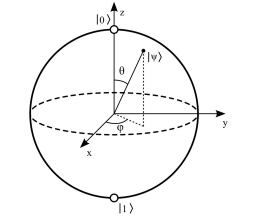
\includegraphics[scale=0.5]{chapters/res/bloch-sphere.png}
    \caption{Bloch Sphere (Felix Bloch)}
\end{figure}

\subsection{Single qubit gates}

Principles of \underline{time evolution}: The quantum state $\ket{\psi}$ at current
time point $t$ transitions to a new quantum state $\ket{\psi'}$ at a later time point
$t' > t$. \newline
Transition described by a complex unitary matrix $U$:
\begin{equation}
    \ket{\psi'} = U \cdot \ket{\psi}
\end{equation}

\begin{figure}[h!]
    \centering
    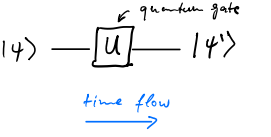
\includegraphics[scale=0.5]{chapters/res/circuit_time_evolution.png}
    \caption{Circuit notation}
\end{figure}

Notes: 
\begin{itemize}
    \item Circuit is read from left to right, but matrix times vector ($U\ket{\psi}$) from right to left.
    \item $U$ preserves normalization
\end{itemize}

Examples:
\begin{itemize}
    \item Quantum analogue of the classical NOT gate ($0 \leftrightarrow 1$) flip
    $\ket{0} \leftrightarrow \ket{1}$ leads to Pauli-X gate:
    \begin{equation}
        X \equiv \sigma_1 = \begin{pmatrix}
            0 & 1 \\
            1 & 0
        \end{pmatrix}
    \end{equation}

    Check: $X\ket{0} = \begin{pmatrix}
            0 & 1 \\
            1 & 0
        \end{pmatrix} \begin{pmatrix}0 \\ 1 \end{pmatrix} = \ket{1}$ and 
        $X\ket{1} = \begin{pmatrix}
            0 & 1 \\
            1 & 0
        \end{pmatrix} \begin{pmatrix}1 \\ 0 \end{pmatrix} = \ket{0} 
        \quad \color{green}\checkmark $
    
    \item Pauli-Y gate: 
    \begin{equation}
        Y \equiv \sigma_2 = \begin{pmatrix}
            0 & -i \\
            i & 0
        \end{pmatrix}
    \end{equation}

    \item Pauli-Z gate: 
    \begin{equation}
        Z \equiv \sigma_3 = \begin{pmatrix}
            1 & 0 \\
            0 & -1
        \end{pmatrix}
    \end{equation}

    Z leaves $\ket{0}$ unchanged, but flips the sign of the coefficient of $\ket{1}$.
    Recall the Bloch Sphere representation:
    \begin{equation*}
        \ket{\psi} = \cos{\frac{\vartheta}{2}} \cdot \ket{0} + e^{i\varphi} \sin{\frac{\vartheta}{2}} \cdot \ket{1}
    \end{equation*} 

    Then
    \begin{align*}
        Z \ket{\psi} &= \cos{\frac{\vartheta}{2}} \cdot \ket{0} {\color{red}\text{ }-\text{ }}
            e^{i\varphi} \sin{\frac{\vartheta}{2}} \cdot \ket{1} \\
        %
        &\stackrel{e^{i\pi} = -1}{=} \cos{\frac{\vartheta}{2}} \cdot \ket{0} + 
            \underbrace{e^{i\pi} e^{i\varphi}}_{e^{i(\varphi + \pi)}} \sin{\frac{\vartheta}{2}} \cdot \ket{1}
    \end{align*}

    $\leadsto$ new Bloch Sphere angles: $\vartheta' = \vartheta, \varphi = \varphi + \pi$ 
    (rotating by $\pi = 180^\circ$ around z-axis) \newline
    X, Y, Z gates are called \underline{Pauli matrices}.
    The \underline{Pauli vector} $\vec{\sigma} = (\sigma_1, \sigma_2, \sigma_3) = (X, Y, Z)$
    is a vector of $2 \times 2$ matrices.

    \item Hadamard Gate:
    \begin{equation*}
        H = \frac{1}{\sqrt{2}}  \begin{pmatrix}
            1 & 1 \\
            1 & -1
        \end{pmatrix}
    \end{equation*}

    \begin{figure}[h]
        \centering
        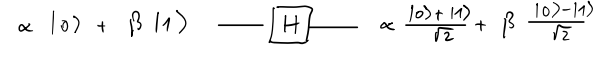
\includegraphics[scale=0.5]{chapters/res/hadamard-gate-circuit.png}
        \caption{Hadamard Gate}
    \end{figure}

    \item Phase Gate:
    \begin{equation*}
        S = \begin{pmatrix}
            1 & 0 \\
            0 & i
        \end{pmatrix}
    \end{equation*}

    \item T Gate:
    \begin{equation*}
        T = \begin{pmatrix}
            1 & 0 \\
            0 & e^{i\pi/4}
        \end{pmatrix}
    \end{equation*}
    Note: $T^2 = S$ since $(e^{i \pi /4})^2 = e^{i\pi/2} = i$
\end{itemize}


Pauli matrices satisfy:
\begin{enumerate}
    \item $\sigma^{2}_{j} = I$ (identifity) for $j = 1,2,3$
    \item $\sigma_j \cdot \sigma_k = - \sigma_k \sigma_j$ for all $j \neq k$
    \item ${\color{blue} [} \sigma_j, \sigma_k {\color{blue} ]} :=
        \underbrace{\sigma_j \sigma_k - \sigma_k \sigma_j}_{\text{Commutator}} = 
        2 i \sigma_l$ for $(j,k,l)$ a cyclic permutation of (1,2,3).
\end{enumerate}

General definition of \underline{matrix exponential}

\begin{equation}
    exp(A) \equiv e^A = \sum_{k = 0}^{\infty} \frac{1}{k!}A^k, \quad A \in \mathbb{C}^{n \times n}
\end{equation}

Special case: $A^2 = I, x \in \mathbb{R}$
\begin{align*}
    e^{i A x} &= \underbrace{\sum_{k = 0}^{\infty} \frac{1}{(2k)!} (ix)^{2k} 
        \underbrace{A^{2k}}_{(A^2)^k = I^k = I}}_\text{even} +
        \underbrace{\sum_{k = 0}^{\infty} \frac{1}{(2k + 1)!} (ix)^{2k + 1} 
            \underbrace{A^{2k+1}}_{(A^2)^k \cdot A = I^k \cdot A= A}}_\text{odd} \\
        &= \underbrace{\sum_{k = 0}^{\infty} \frac{1}{(2k)!} (-1)^k x^{2k}}_{ = \cos{x}} \cdot I +
        \underbrace{\sum_{k = 0}^{\infty} \frac{1}{(2k + 1)!} (-1)^k x^{2k + 1}}_{=i \sin{x}} \cdot A\\
        &= \cos{x} \cdot I + i \sin{x} A
\end{align*}
(generalizes Euler's formula $e^{ix} = \cos{x} + i \sin{x}$)
\newline

This can be used to define the following \underline{rotation operators} via the
Pali matrices. Let $\vartheta \in \mathbb{R}$:

\begin{align}
    R_x(\vartheta) &:= e^{-i \vartheta X / 2} 
        = \cos{\frac{\vartheta}{2}} I - i \sin{\frac{\vartheta}{2}} X 
        = \begin{pmatrix}
            \cos{\frac{\vartheta}{2}} & -i \sin{\frac{\vartheta}{2}} \\
            -i \sin{\frac{\vartheta}{2}} & \cos{\frac{\vartheta}{2}}
        \end{pmatrix} \\
    %
    R_y(\vartheta) &:= e^{-i \vartheta Y / 2} 
        = \cos{\frac{\vartheta}{2}} I - i \sin{\frac{\vartheta}{2}} Y 
        = \begin{pmatrix}
            \cos{\frac{\vartheta}{2}} & -\sin{\frac{\vartheta}{2}} \\
            \sin{\frac{\vartheta}{2}} & \cos{\frac{\vartheta}{2}}
        \end{pmatrix} \\ 
    R_z(\vartheta) &:= e^{-i \vartheta Z / 2} 
        = \cos{\frac{\vartheta}{2}} I - i \sin{\frac{\vartheta}{2}} Z
        = \begin{pmatrix}
            e^{-i \vartheta / 2} & 0 \\
            0 & e^{i \vartheta / 2}
        \end{pmatrix}
\end{align} 
\newpage


General case: Rotation about an axis $\vec{v} \in \mathbb{R}^3$
(normalized such that $\norm{\vec{v}}) = \sqrt{v_1^2 + v_2^2 + v_3^3} = 1$): \newline
using the notation:

\begin{equation}
    \braket{\vec{v}}{\vec{\sigma}} 
        = \vec{v} \cdot \vec{\sigma} 
        = v_1 \sigma_1 + v_2 \sigma_2 + v_3 \sigma_3
        = \begin{pmatrix}
            v_3 && v_1 - i v_2 \\
            v_1 + i v_2 && -v_3
        \end{pmatrix}
\end{equation}

It holds that $(\vec{v} \cdot \vec{\sigma})^2 = I$.

We define the rotation operator around axis $\vec{v}$ as 
\begin{equation}
    R_v(\vartheta) := e^{-i \vartheta (\vec{v} \cdot \vec{\sigma}) / 2} 
        = \cos{\frac{\vartheta}{2}} I - i \sin{\frac{\vartheta}{2}} (\vec{v} \cdot \vec{\sigma})
\end{equation}

Note: $R_x$, $R_y$, $R_z$ are special cases corresponding to $\vec{v} = (1, 0, 0)$, 
$\vec{v} = (0, 1, 0)$, and $\vec{v} = (0, 0, 1)$. \newline 

Can derive that the Bloch Sphere representaiton of $R_{\vec{v}}(\vartheta)$ 
is a "conventional" rotation (in three dimensions) by angle $\vartheta$ about 
axis $\vec{v}$.

\begin{figure}[h]
    \centering
    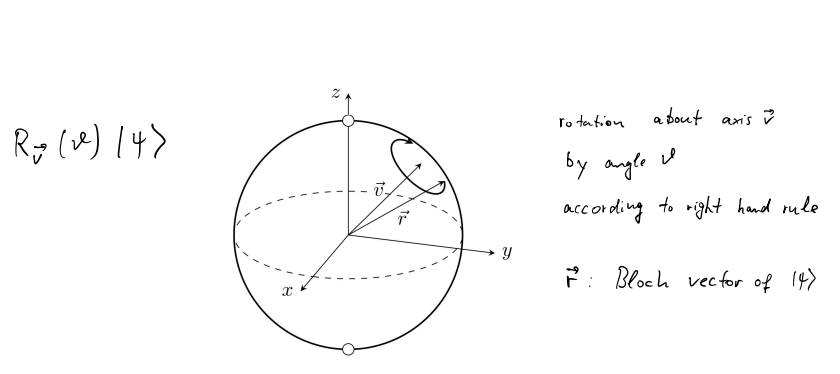
\includegraphics[scale=0.5]{chapters/res/bloch-sphere-rotation.png}
    \caption{Circuit notation}
\end{figure}


\underline{Z-Y decomposition} of an arbitrary $2 \times 2$ unitary matrix: \newline
For any unitary matrix $U \in \mathbb{C}^{n \times n}$ there exist real numbers
$\alpha, \beta, \gamma, \delta \in \mathbb{R}$ such that

\begin{equation}
    U = e^{i \alpha} \underbrace{\begin{pmatrix}
        e^{-i \beta / 2} & 0 \\
        0 & e^{i \beta / 2} 
    \end{pmatrix}}_{R_z(\beta)} \cdot 
    \underbrace{\begin{pmatrix}
        \cos{\frac{\gamma}{2}} & -\sin{\frac{\gamma}{2}} \\
        \sin{\frac{\gamma}{2}} & \cos{\frac{\gamma}{2}}
    \end{pmatrix}}_{R_y(\gamma)} \cdot 
    \underbrace{\begin{pmatrix}
        e^{-i \delta / 2} & 0 \\
        0 & e^{i \delta / 2} 
    \end{pmatrix}}_{R_z(\delta)}
\end{equation}

\subsection{Multiple qubits}

So far: Single qubits, superposition of basis states $\ket{0}$ and $\ket{1}$.
For two qubits, this generalizes to $\{\ket{00}, \ket{01}, \ket{10}, \ket{11}\}$. \newline

General two-qubit state:
\begin{equation}
    \ket{\psi} = \alpha_{00} \ket{00} + \alpha_{01} \ket{01} + \alpha_{10} \ket{10} + \alpha_{11} \ket{11}
\end{equation}
with amplitudes $\alpha_{ij} \in \mathbb{C}$ such that
\begin{equation}
    \abs{\alpha_{00}}^2  + \abs{\alpha_{01}}^2  + \abs{\alpha_{10}}^2  + \abs{\alpha_{11}}^2 = 1 
    \quad \text{(normalization).}
\end{equation}

Can identify the basis states with unit vectors:

\begin{equation}
    \ket{00} = \begin{pmatrix*}
        1 \\ 0 \\ 0 \\ 0
    \end{pmatrix*} \quad
    \ket{01} = \begin{pmatrix*}
        0 \\ 1 \\ 0 \\ 0
    \end{pmatrix*} \quad
    \ket{10} = \begin{pmatrix*}
        0 \\ 0 \\ 1 \\ 0
    \end{pmatrix*} \quad
    \ket{11} = \begin{pmatrix*}
        0 \\ 0 \\ 0 \\ 1
    \end{pmatrix*} \quad
\end{equation}

Thus: 
\begin{equation}
    \ket{\psi} = \begin{pmatrix*}
        \alpha_{00} \\ \alpha_{01} \\ \alpha_{10} \\ \alpha_{11} 
    \end{pmatrix*} \in \mathbb{C}^4
\end{equation}

What happens if we measure only one qubit of a two-qubit state?
Say we measure the first qubit: Obtain result
\begin{align*}
    0 &\quad \text{with probability} \quad \abs{\alpha_{00}}^2 + \abs{\alpha_{01}}^2 \\ 
    1 &\quad \text{with probability} \quad \abs{\alpha_{10}}^2 + \abs{\alpha_{11}}^2
\end{align*}

Wavefunction directly after measurement:
\begin{align*}
    &\text{if measured 0:} \quad \ket{\psi'} 
        = \frac{\alpha_{00}\ket{00} + \alpha_{01}\ket{01}}{\sqrt{\abs{\alpha_{00}}^2 + \abs{\alpha_{01}}^2}} \\
    &\text{if measured 1:} \quad \ket{\psi'} 
        = \frac{\alpha_{10}\ket{10} + \alpha_{11}\ket{11}}{\sqrt{\abs{\alpha_{10}}^2 + \abs{\alpha_{11}}^2}} \\
\end{align*}


Mathematical formalism for constructing two qubit states: Tensor product of vector space. \newline
Can combine two (arbitrary) vector spaces $V$ and $W$ to form the \underline{tensor product}
$V \otimes W$. \\
The elements of $V \otimes W$ are linear combinations of "tensor products" 
$\ket{v} {\color{blue} \otimes} \ket{w}$ consisting of elements $\ket{v} \in V$ and  $\ket{w} \in W$. \\

Example: Let $V = \mathbb{C}^2$ and $W = \mathbb{C}^2$ be the single qubit spaces with basis
$\{\ket{0}, \ket{1}\}$, then

\begin{equation*}
    \underbrace{\frac{1}{2} \ket{0} {\color{blue} \otimes} \ket{0}}_{=\ket{00}} + 
    \underbrace{\frac{5i}{7} \ket{1} {\color{blue} \otimes} \ket{0}}_{=\ket{10}} 
    \in V \otimes W
\end{equation*}

Let $\{\ket{i}_v : i = 1, ... ,m\}$ be a basis of of V, and 
let $\{\ket{j}_w : j = 1, ... ,n\}$ be a basis of of W, then

\begin{equation*}
    \{\ket{i}_v {\color{blue}\otimes} \ket{j}_w : i = 1,...,m, j = 1,...,n \}    
\end{equation*}
is a basis of $V {\color{blue} \otimes} W$.
In particular, $dim(V \otimes W) = dim(V) \cdot dim(W)$.\\ 
Note: $\ket{i}_v {\color{blue}\otimes} \ket{j}_w$ is also written as $\ket{ij}$. \\

Basic properties of tensor product:
\begin{itemize}
    \item $\forall \ket{v} \in V, \ket{w} \in W \land \alpha \in \mathbb{C}:$
    \begin{equation}
        \alpha (\ket{v} \otimes \ket{w}) 
            = (\alpha \ket{0}) \otimes \ket{w} 
            = \ket{v} \otimes (\alpha \ket{w})
    \end{equation}

    \item $\forall \ket{v_1}, \ket{v_2} \in V \land \ket{w} \in W:$
    \begin{equation}
        (\ket{v_1} + \ket{v_2}) \otimes \ket{w} 
            = \ket{v_1} \otimes \ket{w} + \ket{v_2} \otimes \ket{w}
    \end{equation}

    \item $\forall \ket{v} \in V \land \ket{w_1}, \ket{w_2} \in W:$
    \begin{equation}
        \ket{v} \otimes (\ket{w_1} + \ket{w_2})
            = \ket{v} \otimes \ket{w_1} + \ket{v} \otimes \ket{w_2}
    \end{equation}
\end{itemize}

Vector notation using standard basis, e.g.
\begin{align*}
    \ket{v} &= v_1\ket{0} + v_2\ket{1} = \begin{pmatrix*}
        v_1 \\ v_2
    \end{pmatrix*} \\
    \ket{w} &= w_1\ket{0} + w_2\ket{1} = \begin{pmatrix*}
        w_1 \\ w_2
    \end{pmatrix*} \\
    \ket{v} \otimes \ket{w} &= (v_1\ket{0} + v_2\ket{1}) \otimes (w_1\ket{0} + w_2\ket{1}) \\
    &= v_1 w_1 \ket{00} + v_1 w_2 \ket{01} + v_2 w_1 \ket{10} + v_2 w_2 \ket{11}
\end{align*}

Thus: 
\begin{equation*}
    \begin{pmatrix*}
        v_1 \\ v_2
    \end{pmatrix*} \otimes
    \begin{pmatrix*}
        w_1 \\ w_2
    \end{pmatrix*} = 
    \begin{pmatrix*}
        v_1 w_1 \\ v_1 w_2 \\ v_2 w_1 \\ v_2 w_2
    \end{pmatrix*}
\end{equation*}


Note: Not every element of $V \otimes W$ can be written in the form $\ket{v} \otimes \ket{w}$,
for example the Bell state
\begin{equation*}
    \ket{\psi} = \frac{1}{\sqrt{2}} (\ket{00} + \ket{11}).
\end{equation*}

Assuming that $V$ and $W$ have an inner product $\braket{\cdot}{\cdot}$, define inner product
on $V \otimes W$ by

\begin{equation}
    \braket{\sum_j \alpha_j \ket{v_j} \otimes \ket{w_j}}
        {\sum_k \beta_k \ket{v_k} \otimes \ket{w_k}} :=
    \sum_j \sum_k \alpha_j^* \beta_k \braket{v_j}{v_k}\cdot \braket{w_j}{w_k}
\end{equation}


Generalization to $n$ qubits: $2^n$ computational basis states
\begin{equation*}
    \{\underbrace{\ket{0, ..., 0}}_{\text{length $n$}}, \ket{0, ..., 0, 1}, ... \ket{1,...,1}\}
\end{equation*}

Thus: General n-qubit quantum state, also denoted as "quantum register", given by:

\begin{equation}
    \ket{\psi} = \sum_{x_0 = 0}^1 \sum_{x_1 = 0}^2 \cdots \sum_{x_{n-1}}^1 \alpha_{x_n-1,..., x_1, x_0}
        \cdot \ket{x_{n-1},..., x_1 x_0}
\end{equation}

with $\alpha_x \in \mathbb{C}$ for all $x \in \{0, ..., 2^n - 1\}$, such that 
$\norm{\psi}^2 = \sum_{x = 0}^{2^n - 1} \abs{\alpha_x}^2 = 1$ (normalization).

$\leadsto$ In general \textit{"hard"} to simulate on classical computer (for large $n$) due to "curse of dimensionality". \\
Vector space as tensor products: 
$\underbrace{\mathbb{C}^2 \otimes \cdots \otimes \mathbb{C}^2}_{\text{$n$ times}} 
= (\mathbb{C}^2)^{\otimes n} = \mathbb{C}^{(2^n)}$

\subsection{Multiple qubit gates}

As for single qubits, an operation on multiple qubits is described by an unitary matrix $U$.
For $n$ qubits: $U \in \mathbb{C}^{2^n \times 2^n}$
\newpage
%
Example: \underline{controlled-NOT} gate (also CNOT): \\
two qubits: {\color{orange}control} and target, target qubit gets flipped if {\color{orange}control} is 1: \\

\begin{equation*}
    \ket{{\color{orange}0}0} \mapsto \ket{00}, 
    \quad \ket{{\color{orange}0}1} \mapsto \ket{01}, 
    \quad \ket{{\color{orange}1}0} \mapsto \ket{11}, 
    \quad \ket{{\color{orange}1}1} \mapsto \ket{11}
\end{equation*}

Can be expressed as
\begin{equation}
    \ket{a, b} \mapsto \ket{a, a \oplus b} \quad \forall a, b \in \{0, 1\}
\end{equation}
, where $\oplus$ is the addition modulo 2.

\begin{figure}[h]
    \centering
    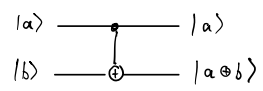
\includegraphics[scale=0.5]{chapters/res/cnot-circuit.png}
    \caption{CNOT circuit notation}
\end{figure}

Matrix representation:

\begin{equation}
    U_{CNOT} = \begin{pmatrix*}
        1 && 0 && 0 && 0 \\
        0 && 1 && 0 && 0 \\
        0 && 0 && \color{red} 0 && \color{red} 1 \\
        0 && 0 && \color{red} 1 && \color{red} 0 \\
    \end{pmatrix*}
\end{equation},
with the Pauli-X matrix $X = \begin{pmatrix*}
        \color{red} 0 && \color{red} 1 \\
        \color{red} 1 && \color{red} 0 \\
\end{pmatrix*}$.
 
\begin{figure}[h]
    \centering
    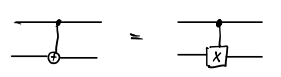
\includegraphics[scale=0.5]{chapters/res/cnot-alternative-circuit.png}
    \caption{Alternative CNOT circuit notation}
\end{figure}

Can generalize Pauli-X to any unitary operator U acting on target qubit $\leadsto$ 
\textbf{controlled-U gate}:

\begin{equation*}
    \ket{{\color{orange}0}0} \mapsto \ket{00}, 
    \quad \ket{{\color{orange}0}1} \mapsto \ket{01}, 
    \quad \ket{{\color{orange}1}0} \mapsto \ket{1} {\color{blue} \otimes} (U\ket{0}), 
    \quad \ket{{\color{orange}1}1} \mapsto \ket{1} {\color{blue} \otimes} (U\ket{1})
\end{equation*}

\begin{figure}[H]
    \centering
    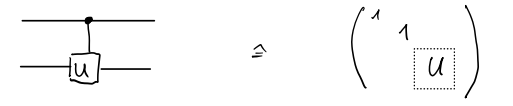
\includegraphics[scale=0.5]{chapters/res/contolled-u-gate-circuit.png}
    \caption{Controlled-U gate}
\end{figure}

\begin{figure}[H]
    \centering
    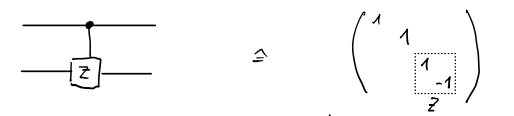
\includegraphics[scale=0.5]{chapters/res/controlled-z-gate-circuit.png}
    \caption{Example: Controlled-Z gate}
\end{figure}

\begin{figure}[H]
    \centering
    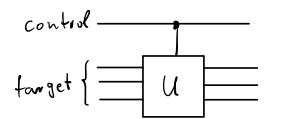
\includegraphics[scale=0.5]{chapters/res/controlled-u-multiple-targets.png}
    \caption{Controlled-U for multiple target qubits}
\end{figure}

Note: Single qubit and CNOT gates are \underline{universal}: They can be used to implement an 
arbitraty unitray operation on $n$ qubits (Quantum analogue of univerisity of classical NAND gate).
Proof in Nielsen and Chuang section 4.5.

\begin{figure}[H]
    \centering
    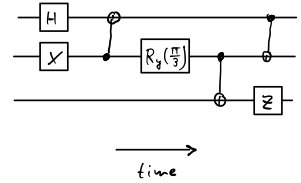
\includegraphics[scale=0.5]{chapters/res/example-qubit-single-qubit-gates-cnot.png}
    \caption{Example of a circuit lousisting only of single qubit gates and CNOTs}
\end{figure}

\subsubsection{Matrix Kronecker Products}
Matrix representation of single qubit gates acting in parallel:

\begin{figure}[H]
    \centering
    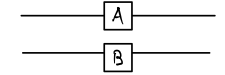
\includegraphics[scale=0.5]{chapters/res/parallel-circuit.png}
\end{figure}

Operation on basis states: $a, b \in \{0, 1\}$:
\begin{equation}
    \ket{a, b} \mapsto (A\ket{a}) \otimes (B\ket{b})
\end{equation}

Example: $A = I$ (identity), $B = Y$
\begin{align*}
    \ket{00} &\mapsto \ket{0} \otimes (Y\ket{0}) = {\color{purple}i}\ket{01} \\
    \ket{01} &\mapsto \ket{0} \otimes (Y\ket{1}) = {\color{green}-i} \ket{00} \\
    \ket{10} &\mapsto \ket{1} \otimes (Y\ket{0}) = i \ket{11} \\
    \ket{11} &\mapsto \ket{1} \otimes (Y\ket{1}) = -i \ket{10}
\end{align*}

Matrix representation:
\begin{equation*}
    \begin{pmatrix*}
        0 && \color{green} -i && 0 && 0 \\
        \color{purple} i && 0 && 0 && 0 \\
        0 && 0 && 0 && -i \\
        0 && 0 && i && 0 \\
    \end{pmatrix*} =
    \begin{pmatrix*}
        Y && 0 \\
        0 && Y
    \end{pmatrix*} = 
    I \otimes Y
\end{equation*}

\begin{figure}[H]
    \centering
    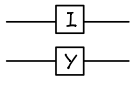
\includegraphics[scale=0.5]{chapters/res/parallel-circuit-i-y.png}
    \caption{Circuit notation}
\end{figure}

General formula: \underline{Kronecker product} (matrix representation of tensor products of operators)

\begin{equation}
    A \otimes B = \begin{pmatrix*}
        a_{11} B && a_{12} B && \cdots && a_{1n} B \\
        a_{21} B && a_{22} B && \cdots && a_{2n} B \\
        \vdots && \vdots && \ddots && \vdots \\
        a_{m1} B && a_{m2} B && \cdots && a_{mn} B \\
    \end{pmatrix*} \in
    \mathbb{C}^{mp \times nq} 
\end{equation}

for all $ A \in \mathbb{C}^{m \times n}$ and $B \in \mathbb{C}^{p \times q}$.

\begin{figure}[H]
    \centering
    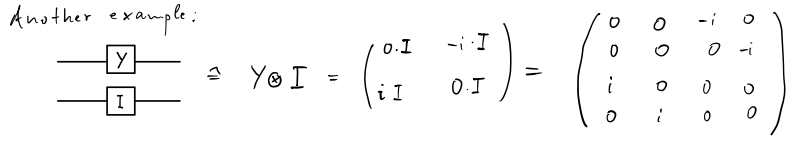
\includegraphics[scale=0.48]{chapters/res/kronecker-another-example.png}
\end{figure}

\begin{figure}[H]
    \centering
    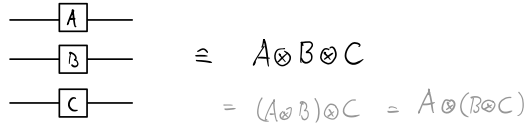
\includegraphics[scale=0.5]{chapters/res/kronecker-generlization-3-tensors.png}
    \caption{Generalization to arbitrary number of tensor factors possible}
\end{figure}

Basic properties:
\begin{enumerate}
    \item $(A \otimes B)^* = A^* \otimes B^*$ (elementwise complex conjugation)
    \item $(A \otimes B)^T = A^T \otimes B^T$ (transposition)
    \item $(A \otimes B)^\dag = A^\dag \otimes B^\dag$
    \item $(A \otimes B) \otimes C = A \otimes (B \otimes C)$ (associative property)
    \item $(A \otimes B) \cdot (C \otimes D) 
        = (A \cdot C) \otimes (B \cdot D)$ (for matrix of compatible dimensions)
        \begin{figure}[H]
            \centering
            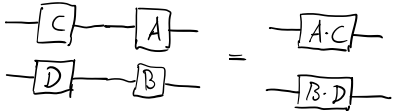
\includegraphics[scale=0.5]{chapters/res/kronecker-properties.png}
        \end{figure}
    \item Kronecker product of Hermitian matrices is Hermitian.
    \item Kronecker product of unitary matrices is unitary (follows from 3. and 5.)
\end{enumerate}

\subsection{Quantum measurement}
Review: measurement of a single qubit $\ket{\psi} = \alpha\ket{0} + \beta{\ket{1}}$ with
resepct to the computational basis $\{\ket{0}, \ket{1}\}$.

\begin{figure}[H]
    \centering
    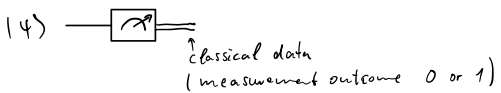
\includegraphics[scale=0.5]{chapters/res/quantum-measurement.png}
\end{figure}

Linear algebra: Can switch to a different (orthonormal) basis to represent a qubit, e.g.
\begin{align*}
    \ket{+} &= \frac{\ket{0} + \ket{1}}{\sqrt{2}} = \frac{1}{\sqrt{2}} \begin{pmatrix*}1 \\ 1\end{pmatrix*} \\
    \ket{-} &= \frac{\ket{0} - \ket{1}}{\sqrt{2}} = \frac{1}{\sqrt{2}} \begin{pmatrix*}1 \\ -1\end{pmatrix*}
\end{align*}

Representation of $\ket{\psi}$ w.r.t $\{\ket{+}, \ket{-}\}$ basis:
\begin{equation*}
    \alpha \ket{0} + \beta \ket{1} 
        = \alpha \frac{\ket{+} + \ket{-}}{\sqrt{2}} + \beta \frac{\ket{+} - \ket{-}}{\sqrt{2}}
        = \frac{\alpha + \beta}{\sqrt{2}} \ket{+} + \frac{\alpha - \beta}{\sqrt{2}} \ket{-}
\end{equation*}

Can perform measurement with resepct to orthonormal basis $\{\ket{+}, \ket{-}\}$, will obtain result
\begin{align*}
    + \quad &\text{with probability} \quad \frac{\abs{\alpha + \beta}^2}{2} \\
    - \quad &\text{with probability} \quad \frac{\abs{\alpha - \beta}^2}{2}
\end{align*}

Wavefunction collapse: immediately after the measurement, qubit will be in the state $\ket{+}$ if 
measured "+", likewise in the state $\ket{-}$ if measured "-".

\begin{figure}[H]
    \centering
    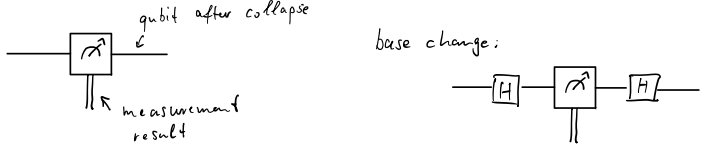
\includegraphics[scale=0.5]{chapters/res/measurement-collapse-basis.png}
\end{figure}

In general given an orthonormal basis $\{\ket{u_1}, \ket{u_2}\}$,
one can represent a qubit as $\ket{\psi} = \alpha_1 \ket{u_1} + \alpha_2 \ket{u_1}$
and measure with respect to this orthonormal basis;
will obtain measurement result $u_1$ or $u_2$ with respective probabilities $\abs{\alpha_1}^2$
and $\abs{\alpha_2}^2$.

\subsubsection{Abstract general definition of quantum measurements}
Quantum measurements are described by a collection $\{M_m\}$ of 
\underline{measurement} \underline{operators} acting on the quantum system, with the index $m$ labelling possible 
measurement outcomes. \\
Denoting the quantum state before measurement $\ket{\psi}$, result $m$ occurs with probability
\begin{equation}
    p(m) = \braketmatrix{\psi}{M_m^\dag M_m}{\psi} = \norm{M_m \ket{\psi}}^2
\end{equation}
, state after measurement is:
\begin{equation}
    \frac{M_m \ket{\psi}}{\norm{M_m \ket{\psi}}}
\end{equation}

The measurement operators satisfy the completeness relation

\begin{equation}
    \sum_m M_m^\dag M_m = I
\end{equation}

such that probabilities sum to 1:

\begin{equation}
    \sum_m p(m) 
        = \sum_m \braketmatrix{\psi}{M_m^\dag M_m}{\psi} 
        = \braketmatrix{\psi}{\sum_m M_m^\dag M_m}{\psi} \braket{\psi}{\psi} 
        = 1
\end{equation}
since $\sum_m M_m^\dag M_m = I$. \\
\newline
%
Example: measurement of a qubit $\ket{\psi} = \alpha \ket{0} + \beta \ket{1}$
with respect to computational basis $\{\ket{0}, \ket{\psi}\}$.

\begin{align*}
    M_0 &:= \ket{0} \bra{0} = \begin{pmatrix*}1 \\ 0\end{pmatrix*} (1, 0) = \begin{pmatrix*}
        1 && 0 \\ 0 && 0
    \end{pmatrix*} \\
    %
    M_1 &:= \ket{1} \bra{1} = \begin{pmatrix*}0 \\ 1\end{pmatrix*} (0, 1) = \begin{pmatrix*}
        0 && 0 \\ 0 && 1
    \end{pmatrix*} \\
    \leadsto p(0) &= \braketmatrix{\psi}{M_0^\dag M_0}{\psi} = \braketmatrix{\psi}{M_0}{\psi} = \abs{\alpha}^2 \\
    p(1) &= \braketmatrix{\psi}{M_1^\dag M_1}{\psi} = \braketmatrix{\psi}{M_1}{\psi} = \abs{\beta}^2 \\
\end{align*}

\subsubsection{Projective Measurements}
Projector onto subspace $V$ with orthonormal basis $\{\ket{u_1}, ..., \ket{u_m}\}$:
\begin{align}
    P &= \sum_{j = 1}^m \ket{u_j} \bra{u_j} \\
    P \ket{w} &= \sum_{j = 1}^m \underbrace{\braket{u_j}{w}}_{\text{inner product}}
\end{align}

Relation to spectral decomposition of a normal matrix $A \in \mathbb{C}^{n \times n}$:

\begin{align}
    A &= U \begin{pmatrix*}
        \lambda_1 & & \\
        & \ddots & \\
        & & \lambda_n
    \end{pmatrix*} U^\dag
    = \sum_{j = 1}^n \lambda_j \ket{u_j} \bra{u_j} \\
    &= \sum_{k = 1}^m \widetilde{\lambda_k} P_k \quad 
    \text{with } \{\widetilde{\lambda_1} ... \widetilde{\lambda_m} \} \text{ the distinct eigenvalues}
\end{align}

Definition:
A \underline{projective measurement} is described by an \underline{observable} $M$, 
a Hermitian operator acting on the quantum system.
Spectal decomposition:

\begin{equation}
    M = \sum_m \lambda_m P_m
\end{equation}

with $P_m$: projection onto eigenspace with eigenvalue $\lambda_m$.
The possible outcomes of the measurement correspond to the eigenvalues $\lambda_m$. \\
Probability of getting result $\lambda_m$ when measuring a quantum state $\ket{\psi}$:
\begin{equation}
    p(\lambda_m) = \braketmatrix{\psi}{P_m}{\psi}
\end{equation}

State of the quantum system directly after the measurement:

\begin{equation}
    \frac{P_m \ket{\psi}}{\norm{P_m \ket{\psi}}} = \frac{P_m \ket{\psi}}{\sqrt{p(\lambda_m)}}
\end{equation}

Remarks:
\begin{itemize}
    \item Projective measurements are special cases of general measurement framework
    \item Projective measurements combined with unitary transformations are equivalent to general
    measurement framework, see pages 94, 95 in Nielsen and Chuang.
\end{itemize}

Average value of a projective measurement:
\begin{align}
    \mathbb{E}[M] &= \sum_m \lambda_m p(\lambda_m) = \sum_m \lambda_m \braketmatrix{\psi}{P_m}{\psi} \\
    &= \braketmatrix{\psi}{\sum_m \lambda_m P_m}{\psi} = \braketmatrix{\psi}{M}{\psi} = \langle M \rangle
\end{align}

Corresponding \underline{standard deviation}:
\begin{equation}
   \Delta(M) := \sqrt{\langle M^2 \rangle - \langle M \rangle^2} 
        = \sqrt{\langle (M - \langle M \rangle)^2 \rangle}
\end{equation}